\documentclass[12pt, a4paper]{article}

% ── Codificação e Idioma ─────────────────────────────────────────────────────
\usepackage[utf8]{inputenc}
\usepackage[T1]{fontenc}
\usepackage[brazil]{babel}

% ── Layout ───────────────────────────────────────────────────────────────────
\usepackage[top=3cm, bottom=2.5cm, left=3cm, right=2.5cm]{geometry}
\usepackage{setspace}
\onehalfspacing

% ── Matemática ───────────────────────────────────────────────────────────────
\usepackage{amsmath, amssymb}

% ── Figuras e Tabelas ────────────────────────────────────────────────────────
\usepackage{graphicx}
\usepackage{float}
\usepackage{caption}
\usepackage{subcaption}
\usepackage{booktabs}
\usepackage{multirow}
\usepackage{longtable}
\graphicspath{{reports/figures/}}

% ── Código-fonte ─────────────────────────────────────────────────────────────
\usepackage{listings}
\usepackage{xcolor}
\definecolor{codegray}{rgb}{0.95,0.95,0.95}
\definecolor{codegreen}{rgb}{0.1,0.5,0.1}
\definecolor{codepurple}{rgb}{0.45,0.1,0.6}
\definecolor{codeblue}{rgb}{0.1,0.1,0.8}
\lstset{
  backgroundcolor=\color{codegray},
  basicstyle=\ttfamily\footnotesize,
  keywordstyle=\color{codeblue}\bfseries,
  commentstyle=\color{codegreen}\itshape,
  stringstyle=\color{codepurple},
  breaklines=true,
  frame=single,
  rulecolor=\color{gray!40},
  captionpos=b,
  numbers=left,
  numberstyle=\tiny\color{gray},
  numbersep=8pt,
  showstringspaces=false,
  language=Python,
  literate={á}{{\'a}}1 {é}{{\'e}}1 {í}{{\'i}}1 {ó}{{\'o}}1 {ú}{{\'u}}1
           {ã}{{\~a}}1 {õ}{{\~o}}1 {ç}{{\c{c}}}1 {â}{{\^a}}1 {ê}{{\^e}}1
}

% ── Links ────────────────────────────────────────────────────────────────────
\usepackage[hidelinks, colorlinks=true, linkcolor=blue!60!black,
            citecolor=blue!60!black, urlcolor=blue!60!black]{hyperref}

% ── Cabeçalho ────────────────────────────────────────────────────────────────
\usepackage{fancyhdr}
\pagestyle{fancy}
\fancyhf{}
\rhead{\small GalaxyNet — Classificador Morfológico de Galáxias}
\lhead{\small UESC — Deep Learning Aplicado à Astrofísica}
\cfoot{\thepage}

% ── Miscelânea ───────────────────────────────────────────────────────────────
\usepackage{enumitem}
\usepackage{microtype}
\usepackage{lipsum}

% ─────────────────────────────────────────────────────────────────────────────
\begin{document}

% ── Capa ─────────────────────────────────────────────────────────────────────
\begin{titlepage}
  \centering
  \vspace*{2cm}
  {\Large Universidade Estadual de Santa Cruz --- UESC \par}
  \vspace{0.4cm}
  {\large Departamento de Ciências Exatas e Tecnológicas \par}
  \vspace{3cm}
  {\Huge\bfseries GalaxyNet \par}
  \vspace{0.5cm}
  {\LARGE Classificador Morfológico de Galáxias \par}
  \vspace{0.8cm}
  {\large\itshape Relatório Parcial --- Etapas de Aquisição de Dados,\\
   Análise Exploratória e Pré-processamento \par}
  \vfill
  {\large Disciplina: Deep Learning Aplicado à Astrofísica \par}
  \vspace{0.3cm}
  {\large Prof.\ André Ribeiro \par}
  \vspace{1cm}
  {\large \today \par}
\end{titlepage}

% ── Sumário ──────────────────────────────────────────────────────────────────
\tableofcontents
\newpage

% ─────────────────────────────────────────────────────────────────────────────
\section{Resumo}
% ─────────────────────────────────────────────────────────────────────────────

Este relatório descreve as etapas implementadas até o momento no projeto
\textbf{GalaxyNet}, cujo objetivo é construir um \textit{pipeline} completo de
\textit{Deep Learning} para classificação morfológica automática de galáxias.
O projeto utiliza dados reais do levantamento SDSS DR17 (\textit{Sloan Digital
Sky Survey}, Data Release 17) e rótulos supervisionados do Galaxy Zoo~2.

As etapas concluídas cobrem: (i)~aquisição e mesclagem dos dados fotométricos,
espectroscópicos e morfológicos; (ii)~análise exploratória de dados (EDA);
(iii)~engenharia de \textit{features} tabulares e normalização com
\textit{StandardScaler}; e (iv)~pré-processamento de imagens FITS com
normalização \textit{arcsinh} e redimensionamento via OpenCV.
O catálogo resultante contém 156~galáxias com 15~\textit{features} tabulares
e imagens de resolução $64 \times 64$ pixels em três bandas fotométricas
(\textit{g}, \textit{r}, \textit{i}).

\newpage

% ─────────────────────────────────────────────────────────────────────────────
\section{Introdução}
% ─────────────────────────────────────────────────────────────────────────────

A morfologia das galáxias --- sua forma e estrutura visual --- é um dos
indicadores mais diretos de sua história evolutiva. A classificação morfológica
manual, historicamente baseada na \textbf{Sequência de Hubble} (elípticas,
lenticulares, espirais e irregulares), torna-se inviável diante do volume
produzido por grandes levantamentos modernos, que catalogam dezenas de milhões
de objetos. O \textit{Deep Learning} surge como ferramenta natural para
automatizar esse processo, aprendendo representações visuais e fotométricas
diretamente dos dados.

O projeto GalaxyNet tem como objetivo construir e avaliar três arquiteturas:
\begin{itemize}[leftmargin=2em]
  \item \textbf{MLP} (\textit{Multi-Layer Perceptron}): utiliza exclusivamente
        \textit{features} tabulares derivadas de fotometria e espectroscopia.
  \item \textbf{CNN} (\textit{Convolutional Neural Network}): utiliza imagens
        FITS das galáxias em múltiplas bandas.
  \item \textbf{Modelo Híbrido}: combina os dois ramos anteriores em uma
        arquitetura de dupla entrada.
\end{itemize}

Este relatório cobre as fases 1 e 2 do cronograma --- aquisição de dados,
EDA e pré-processamento --- que constituem a fundação sobre a qual os modelos
serão treinados.

% ─────────────────────────────────────────────────────────────────────────────
\section{Bancos de Dados Utilizados}
% ─────────────────────────────────────────────────────────────────────────────

\subsection{SDSS DR17 --- Dados Fotométricos e Espectroscópicos}

O \textit{Sloan Digital Sky Survey} (SDSS) é um dos levantamentos astronômicos
mais abrangentes já realizados, cobrindo mais de um terço do céu e catalogando
centenas de milhões de objetos. A versão DR17 (\textit{Data Release 17}), aqui
utilizada, é a décima-sétima liberação pública de dados e a mais recente da
fase clássica do SDSS.

Os dados foram obtidos por meio de consulta SQL direta ao servidor
\textit{SkyServer} do SDSS via a biblioteca \texttt{astroquery.sdss}. A consulta
une as tabelas \texttt{PhotoObj} (fotometria) e \texttt{SpecObj} (espectroscopia)
e aplica os seguintes filtros de qualidade:

\begin{itemize}[leftmargin=2em]
  \item \texttt{p.clean = 1}: objetos fotométricos sem artefatos.
  \item \texttt{p.r BETWEEN 14.0 AND 19.5}: magnitude $r$ dentro do intervalo
        de completeza do SDSS.
  \item \texttt{s.z BETWEEN 0.02 AND 0.25}: \textit{redshift} espectroscópico
        em faixa que evita objetos muito próximos (efeitos locais) e muito
        distantes (baixa resolução angular).
  \item \texttt{s.zWarning = 0}: \textit{redshift} medido sem alertas de
        qualidade.
\end{itemize}

As colunas recuperadas estão listadas na Tabela~\ref{tab:sdss_cols}.

\begin{table}[H]
  \centering
  \caption{Colunas recuperadas da consulta ao SDSS DR17.}
  \label{tab:sdss_cols}
  \begin{tabular}{llp{7.5cm}}
    \toprule
    \textbf{Coluna} & \textbf{Tipo} & \textbf{Descrição} \\
    \midrule
    \texttt{objid}       & ID      & Identificador único do objeto no SDSS \\
    \texttt{ra, dec}     & Posição & Ascensão reta e declinação (graus) \\
    \texttt{u, g, r, i, z} & Fotometria & Magnitudes nas cinco bandas ópticas \\
    \texttt{petroRad\_r} & Estrutural & Raio de Petrosian na banda $r$ \\
    \texttt{petroR50\_r} & Estrutural & Raio contendo 50\% do fluxo Petrosian \\
    \texttt{petroR90\_r} & Estrutural & Raio contendo 90\% do fluxo Petrosian \\
    \texttt{deVAB\_r}    & Estrutural & Razão axial (perfil de Vaucouleurs) \\
    \texttt{expAB\_r}    & Estrutural & Razão axial (perfil exponencial) \\
    \texttt{lnLDeV\_r}   & Ajuste & Log-verossimilhança do perfil de Vaucouleurs \\
    \texttt{lnLExp\_r}   & Ajuste & Log-verossimilhança do perfil exponencial \\
    \texttt{lnLStar\_r}  & Ajuste & Log-verossimilhança do perfil estelar \\
    \texttt{fracDeV\_r}  & Estrutural & Fração de fluxo do perfil de Vaucouleurs \\
    \texttt{redshift}    & Espectro & \textit{Redshift} espectroscópico \\
    \texttt{zErr}        & Espectro & Incerteza no \textit{redshift} \\
    \texttt{velDisp}     & Espectro & Dispersão de velocidades estelar (km/s) \\
    \texttt{velDispErr}  & Espectro & Incerteza na dispersão de velocidades \\
    \bottomrule
  \end{tabular}
\end{table}

\subsection{Galaxy Zoo 2 --- Rótulos Morfológicos}

O Galaxy Zoo~2 (GZ2) é um projeto de ciência cidadã no qual voluntários
classificaram visualmente mais de 240.000 galáxias do SDSS em categorias
morfológicas por meio de uma árvore de decisão hierárquica. O arquivo de
dados utilizado é o \texttt{gz2\_hart16.csv} \cite{hart2016}, disponível no
repositório Zenodo (\href{https://zenodo.org/record/3565489}{zenodo.org/record/3565489}).

As colunas relevantes extraídas são frações de votos que expressam o grau de
consenso entre os voluntários para cada característica morfológica
(Tabela~\ref{tab:gz2_cols}).

\begin{table}[H]
  \centering
  \caption{Frações de votos do Galaxy Zoo~2 utilizadas na atribuição de classes.}
  \label{tab:gz2_cols}
  \begin{tabular}{lp{9cm}}
    \toprule
    \textbf{Coluna GZ2} & \textbf{Significado} \\
    \midrule
    \texttt{t01\_..\_a01\_smooth\_fraction}   & Fração de votos ``galáxia lisa'' \\
    \texttt{t01\_..\_a02\_features\_fraction} & Fração de votos ``disco / feições'' \\
    \texttt{t01\_..\_a03\_star\_fraction}     & Fração de votos ``estrela / artefato'' \\
    \texttt{t03\_bar\_a06\_bar\_fraction}     & Fração de votos ``barra presente'' \\
    \texttt{t04\_spiral\_a08\_spiral\_fraction} & Fração de votos ``braços espirais'' \\
    \texttt{total\_votes\_gz2}               & Total de votos por galáxia \\
    \bottomrule
  \end{tabular}
\end{table}

\subsection{Cruzamento Espacial SDSS $\times$ GZ2}

O GZ2 foi produzido com base no SDSS DR7, ao passo que os dados fotométricos
foram obtidos no DR17. Consequentemente, os identificadores de objeto
(\texttt{objid}) dos dois catálogos não são diretamente comparáveis. A solução
adotada foi o \textbf{cruzamento espacial por coordenadas} (\textit{sky cross-match}),
implementado com a função \texttt{SkyCoord.match\_to\_catalog\_sky()} da biblioteca
\texttt{astropy}:

\begin{lstlisting}[caption={Cruzamento espacial entre SDSS e GZ2.}, label=lst:crossmatch]
sdss_coords = SkyCoord(ra=sdss_df['ra'].values * u.deg,
                       dec=sdss_df['dec'].values * u.deg)
gz2_coords  = SkyCoord(ra=gz2_df['gz2_ra'].values * u.deg,
                       dec=gz2_df['gz2_dec'].values * u.deg)

idx, sep2d, _ = sdss_coords.match_to_catalog_sky(gz2_coords)
mask = sep2d.arcsec <= 1.0   # separação máxima: 1 arcsec
\end{lstlisting}

A tolerância de 1~arcsec é padrão em aplicações astronômicas e garante
associações únicas sem ambiguidade, dado que o \textit{seeing} típico do SDSS
é de $\sim1{,}4$~arcsec.

\subsection{Atribuição de Classes Morfológicas}

A partir das frações de votos do GZ2, cada galáxia recebe uma das quatro
classes morfológicas segundo a lógica da Tabela~\ref{tab:classes}, com limites
de confiança \texttt{min\_vote\_fraction = 0.8} e \texttt{min\_total\_votes = 20}.
Galáxias que não atingem esses limiares são descartadas como \texttt{Uncertain}.

\begin{table}[H]
  \centering
  \caption{Regras de atribuição de classe morfológica.}
  \label{tab:classes}
  \begin{tabular}{lp{9cm}}
    \toprule
    \textbf{Classe} & \textbf{Condição} \\
    \midrule
    \texttt{Elliptical}  & $f_\text{smooth} \geq 0{,}8$ e $f_\text{features} < 0{,}8$ \\
    \texttt{Lenticular}  & $f_\text{smooth} \geq 0{,}8$ e $f_\text{features} \geq 0{,}8$ \\
    \texttt{Spiral}      & $f_\text{features} \geq 0{,}8$ e $f_\text{spiral} \geq 0{,}8$ \\
    \texttt{Irregular}   & $f_\text{features} \geq 0{,}8$ e $f_\text{spiral} < 0{,}8$ \\
    \texttt{Uncertain}   & Nenhuma condição acima satisfeita, ou $N_\text{votos} < 20$ \\
    \bottomrule
  \end{tabular}
\end{table}

O catálogo final, armazenado em \texttt{data/processed/merged\_catalog.csv},
contém \textbf{156~galáxias} com \textbf{33~colunas}, distribuídas entre as
classes conforme a Tabela~\ref{tab:dist_classes}.

\begin{table}[H]
  \centering
  \caption{Distribuição de classes no catálogo mesclado.}
  \label{tab:dist_classes}
  \begin{tabular}{lrr}
    \toprule
    \textbf{Classe} & \textbf{$N$} & \textbf{Proporção (\%)} \\
    \midrule
    Elliptical  & 135 & 86,5 \\
    Spiral      &  17 & 10,9 \\
    Irregular   &   4 &  2,6 \\
    \midrule
    \textbf{Total} & \textbf{156} & \textbf{100,0} \\
    \bottomrule
  \end{tabular}
\end{table}

O forte desbalanceamento --- com galáxias elípticas representando 86,5\% da
amostra --- é uma característica real da amostra fotométrica brilhante do SDSS
e precisa ser tratado durante o treinamento dos modelos.

% ─────────────────────────────────────────────────────────────────────────────
\section{Análise Exploratória de Dados (EDA)}
% ─────────────────────────────────────────────────────────────────────────────

A EDA foi conduzida no notebook \texttt{notebooks/01\_eda.ipynb} e produziu
seis figuras (\texttt{fig01}--\texttt{fig06}) salvas em \texttt{reports/figures/}.

\subsection{Estatísticas Descritivas e Qualidade dos Dados}

O catálogo mesclado não apresenta valores nulos em nenhuma das colunas
relevantes para o treinamento. As magnitudes cobrem a faixa $14{,}98 \leq r
\leq 17{,}12$, consistente com o filtro de qualidade aplicado na consulta ao
SDSS. O \textit{redshift} espectroscópico varia entre $z = 0{,}02$ e
$z = 0{,}20$, com mediana $z_\text{med} = 0{,}086$, confirmando que a amostra
é composta por galáxias do universo próximo.

\subsection{Distribuição de Classes e Redshift}

A distribuição fortemente assimétrica de classes (Figura~\ref{fig:eda_classes})
é esperada para amostras selecionadas por magnitude: galáxias elípticas massivas
são mais luminosas e, portanto, mais frequentemente detectadas em surveys de
magnitude limite moderada como o SDSS.

A distribuição de \textit{redshift} por classe (Figura~\ref{fig:eda_redshift})
revela que galáxias espirais e irregulares tendem a ser encontradas em
\textit{redshifts} ligeiramente inferiores ($z \lesssim 0{,}15$) em comparação
às elípticas, sugerindo que espirais brilhantes são mais raras na amostra
selecionada.

\subsection{Diagramas de Cor-Magnitude}

O diagrama cor-magnitude $g-r$ versus $r$ (Figura~\ref{fig:eda_cor}) evidencia
a conhecida \textbf{sequência vermelha} e o \textbf{vale de Hubble}:
\begin{itemize}[leftmargin=2em]
  \item Galáxias elípticas concentram-se em $g-r \approx 0{,}93$,
        característica de populações estelares velhas e ricas em metais.
  \item Galáxias espirais ocupam a região de cor intermediária
        ($g-r \approx 0{,}68$), com formação estelar ativa reduzindo
        o índice de cor.
  \item Galáxias irregulares distribuem-se em cores mais azuis
        ($g-r \approx 0{,}58$), consistente com episódios de formação estelar
        recentes.
\end{itemize}

\subsection{Matriz de Correlação}

A matriz de correlação entre as 15~\textit{features} tabulares revela correlações
esperadas do ponto de vista físico: magnitudes em bandas adjacentes são altamente
correlacionadas ($\rho > 0{,}95$), enquanto \textit{redshift} e dispersão de
velocidades apresentam correlação moderada positiva com as magnitudes ($\rho
\approx 0{,}6$--$0{,}8$), refletindo o viés de seleção de Malmquist.

% ─────────────────────────────────────────────────────────────────────────────
\section{Pré-processamento Tabular (Seção 5.2)}
% ─────────────────────────────────────────────────────────────────────────────

O pré-processamento tabular foi implementado no módulo
\texttt{src/preprocessing.py} e executado no notebook
\texttt{notebooks/02\_preprocessing.ipynb}.

\subsection{Engenharia de Features}

A partir das magnitudes brutas, cinco \textit{features} derivadas foram
construídas e adicionadas ao catálogo (Tabela~\ref{tab:features_derivadas}).

\begin{table}[H]
  \centering
  \caption{Features derivadas criadas durante o pré-processamento tabular.}
  \label{tab:features_derivadas}
  \begin{tabular}{llp{7cm}}
    \toprule
    \textbf{Feature} & \textbf{Fórmula} & \textbf{Interpretação física} \\
    \midrule
    \texttt{u\_g} & $u - g$ & Cor UV-óptico; alto em galáxias velhas \\
    \texttt{g\_r} & $g - r$ & Principal discriminador elíptica/espiral \\
    \texttt{r\_i} & $r - i$ & Cor óptico-NIR próximo \\
    \texttt{i\_z} & $i - z$ & Cor NIR próximo \\
    \texttt{concentration} & $R_{90}/R_{50}$ & Concentração de luz; elípticas: $C > 3$, espirais: $C < 3$ \\
    \bottomrule
  \end{tabular}
\end{table}

O índice de concentração $C = R_{90}/R_{50}$, onde $R_{90}$ e $R_{50}$ são os
raios de Petrosian que encerram 90\% e 50\% do fluxo, respectivamente, é um
estimador clássico da morfologia galáctica \cite{conselice2003}. Galáxias com
perfis de brilho centralmente concentrados (elípticas) apresentam valores de
$C$ tipicamente entre 3{,}5 e 5, enquanto espirais e irregulares mostram $C
\lesssim 3$.

A distribuição dos índices de cor por classe morfológica é apresentada na
Figura~\ref{fig:indices_cor}. Observa-se que o índice $g-r$ é o que melhor
separa as três classes, com elípticas claramente mais vermelhas.

O diagrama cor-concentração (Figura~\ref{fig:cor_conc}) confirma que a
combinação dessas duas quantidades é poderosa para a separação de morfologias:
galáxias elípticas concentram-se no quadrante superior-direito ($g-r > 0{,}8$
e $C > 3$).

\begin{figure}[H]
  \centering
  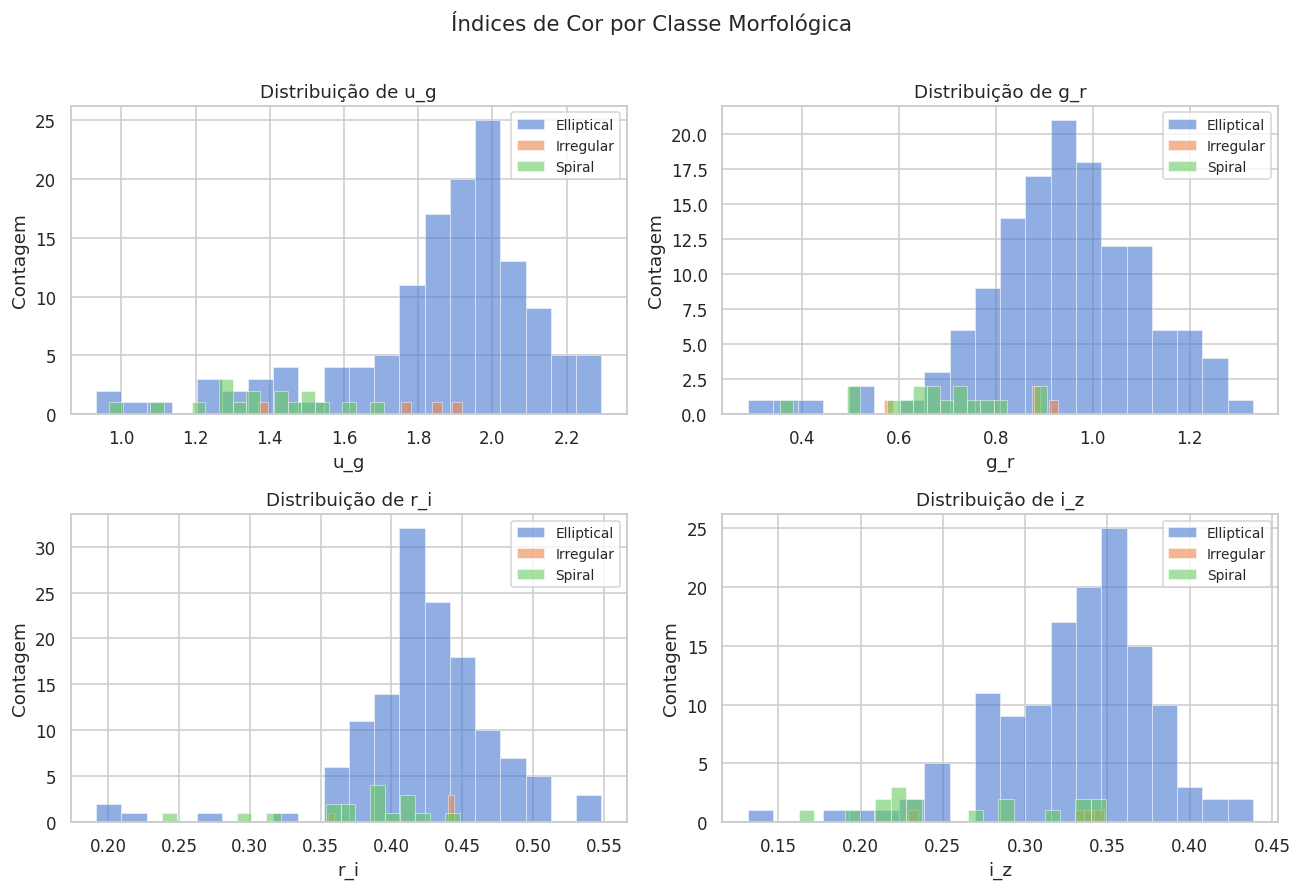
\includegraphics[width=\textwidth]{fig07_indices_cor_distribuicao.png}
  \caption{Distribuição dos índices de cor por classe morfológica.
           Galáxias elípticas apresentam cores consistentemente mais vermelhas
           em todos os índices.}
  \label{fig:indices_cor}
\end{figure}

\begin{figure}[H]
  \centering
  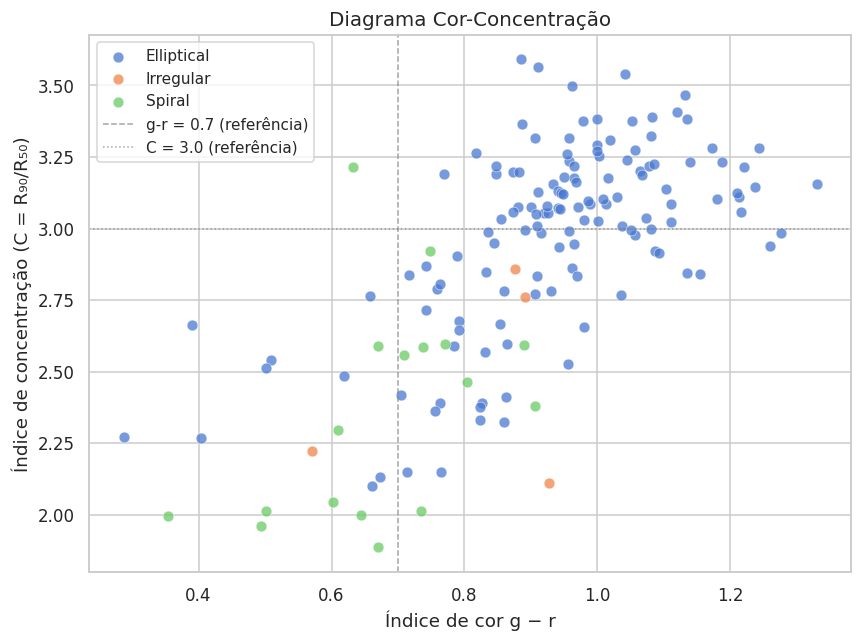
\includegraphics[width=0.75\textwidth]{fig09_cor_concentracao.png}
  \caption{Diagrama cor-concentração ($g-r$ \textit{vs.} $C = R_{90}/R_{50}$).
           As linhas tracejadas marcam os valores de referência $g-r = 0{,}7$
           e $C = 3{,}0$.}
  \label{fig:cor_conc}
\end{figure}

\begin{figure}[H]
  \centering
  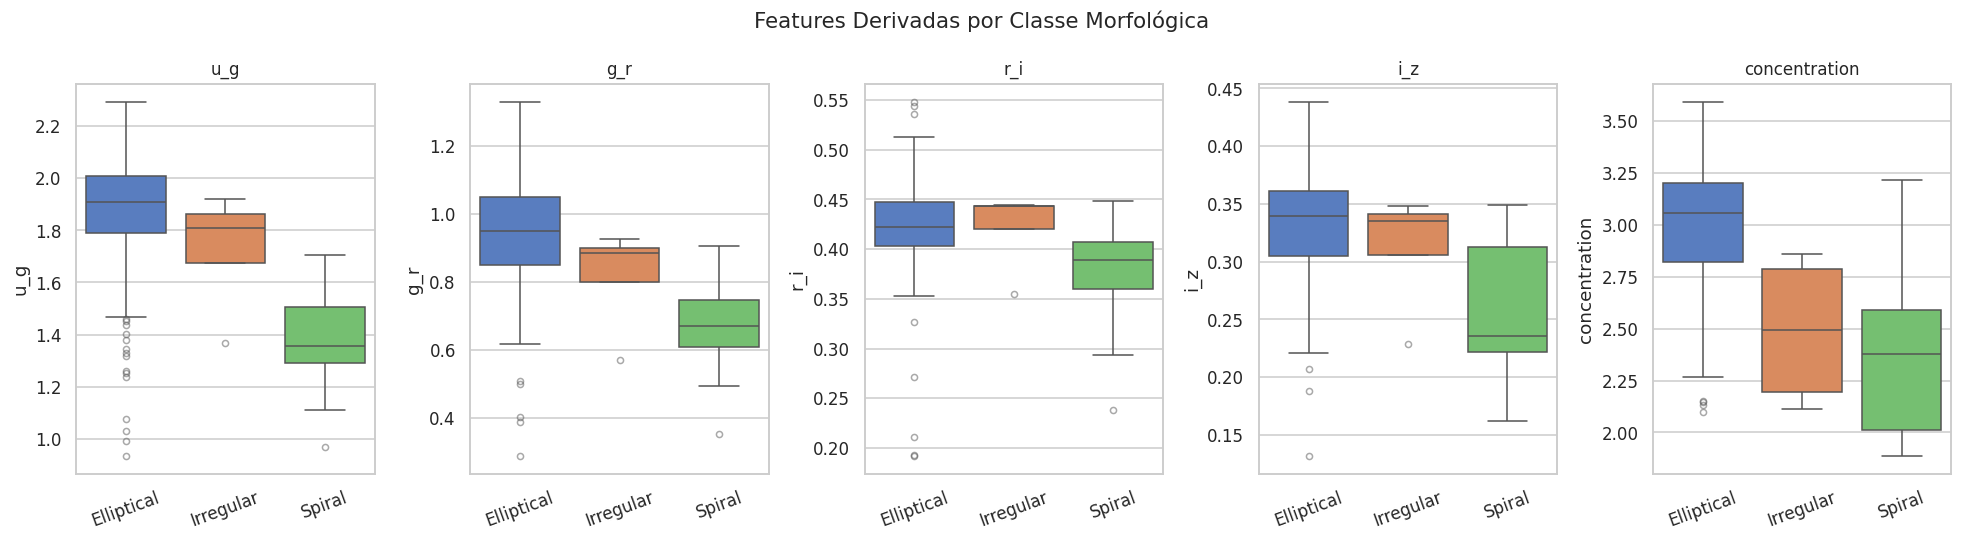
\includegraphics[width=\textwidth]{fig08_features_derivadas_boxplot.png}
  \caption{\textit{Boxplots} das cinco \textit{features} derivadas por classe
           morfológica. A dispersão de cada distribuição reflete a
           heterogeneidade interna das classes.}
  \label{fig:boxplots}
\end{figure}

\subsection{Seleção de Features e Conjunto Final}

O conjunto final de 15~\textit{features} tabulares utilizadas pelo MLP e pelo
ramo tabular do modelo híbrido está listado na Tabela~\ref{tab:features_final}.
A seleção exclui colunas de identificação, coordenadas e frações de votos do
GZ2 (que seriam \textit{data leakage}).

\begin{table}[H]
  \centering
  \caption{Conjunto final de 15 \textit{features} tabulares (\texttt{TABULAR\_FEATURES}).}
  \label{tab:features_final}
  \begin{tabular}{lll}
    \toprule
    \textbf{Grupo} & \textbf{Features} & \textbf{Qtd.} \\
    \midrule
    Magnitudes brutas    & \texttt{u, g, r, i, z}                          & 5 \\
    Índices de cor       & \texttt{u\_g, g\_r, r\_i, i\_z}                 & 4 \\
    Espectroscópicos     & \texttt{redshift, velDisp}                       & 2 \\
    Morfológicos/estruturais & \texttt{concentration, deVAB\_r, expAB\_r, fracDeV\_r} & 4 \\
    \midrule
    \textbf{Total} & & \textbf{15} \\
    \bottomrule
  \end{tabular}
\end{table}

A matriz de correlação entre essas 15~\textit{features} (Figura~\ref{fig:corr})
revela alta colinearidade entre as magnitudes brutas e os índices de cor, o que
é esperado por construção. O \textit{StandardScaler} é aplicado antes do
treinamento, o que elimina o efeito das diferentes escalas mas não a
colinearidade. Caso necessário, uma etapa de PCA pode ser adicionada antes
do MLP.

\begin{figure}[H]
  \centering
  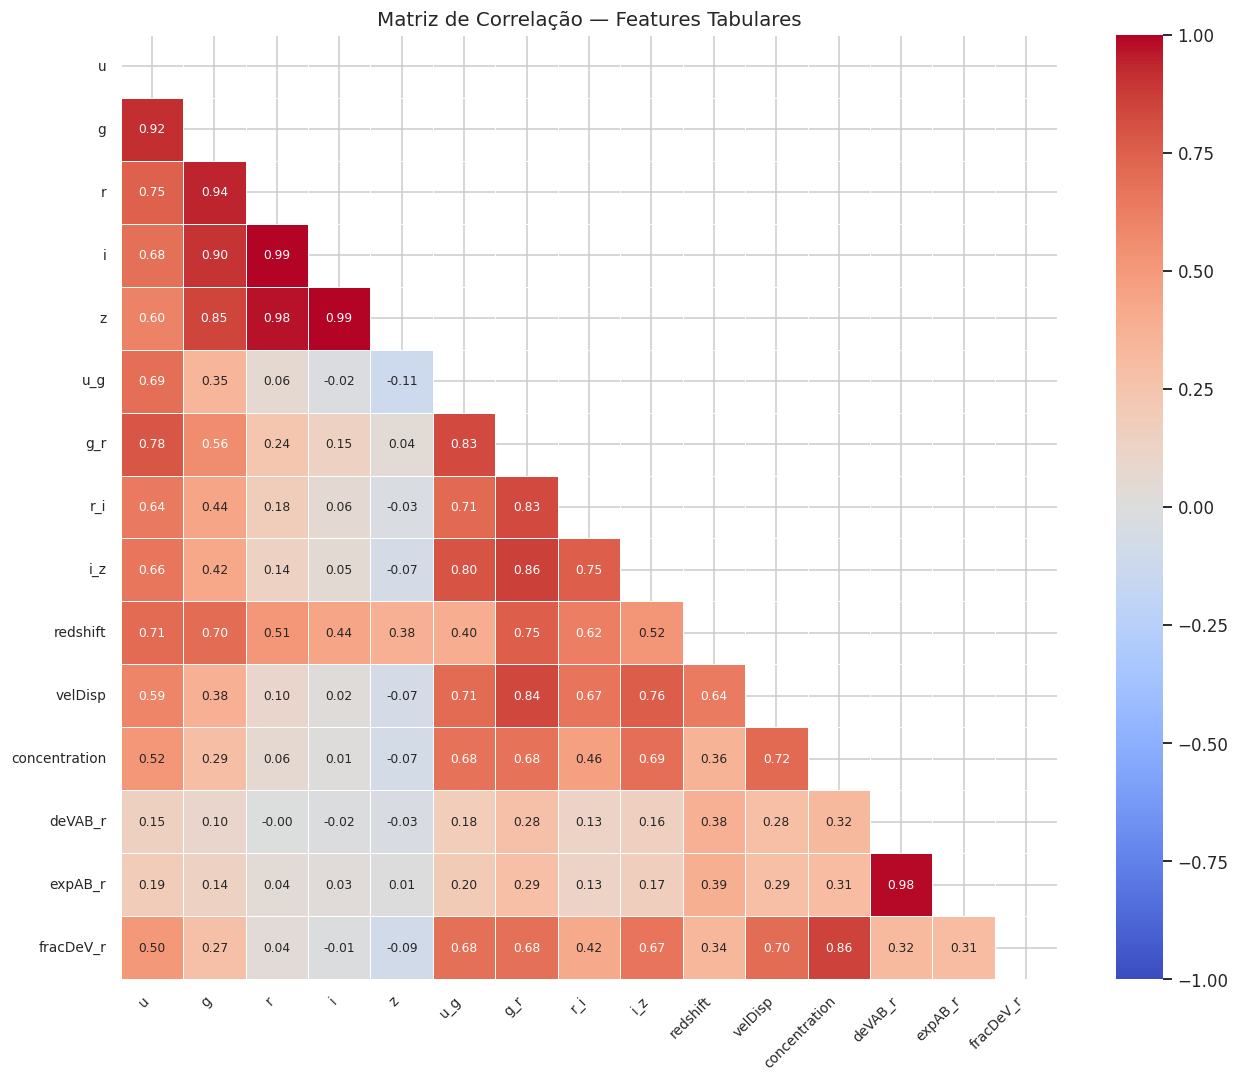
\includegraphics[width=\textwidth]{fig10_correlacao_features_tabulares.png}
  \caption{Matriz de correlação de Pearson entre as 15 \textit{features}
           tabulares. Tons vermelhos indicam correlação positiva, azuis
           indicam correlação negativa.}
  \label{fig:corr}
\end{figure}

\subsection{Normalização com StandardScaler}

A normalização foi realizada com o \texttt{StandardScaler} do
\texttt{scikit-learn}, que transforma cada \textit{feature} $x_j$ segundo:

\begin{equation}
  \tilde{x}_j = \frac{x_j - \mu_j}{\sigma_j}
\end{equation}

onde $\mu_j$ e $\sigma_j$ são a média e o desvio padrão calculados
\textbf{apenas sobre o conjunto de treino}. O scaler ajustado é serializado
em \texttt{data/processed/scaler.pkl} para ser reaplicado sobre os conjuntos
de validação e teste, evitando \textit{data leakage}.

\begin{lstlisting}[caption={Escalonamento das \textit{features} tabulares.}, label=lst:scaler]
scaler   = StandardScaler()
X_scaled = scaler.fit_transform(X_train)   # fit apenas no treino
X_val    = scaler.transform(X_val)         # apenas transform no val
X_test   = scaler.transform(X_test)        # apenas transform no teste
\end{lstlisting}

\subsection{Tratamento do Desbalanceamento de Classes}

A proporção de 86,5\%/10,9\%/2,6\% entre Elliptical/Spiral/Irregular implica
que um classificador trivial que sempre prediz ``Elliptical'' atingiria
$\sim$86\% de acurácia sem aprender nenhuma característica discriminante.
Para mitigar esse problema, adotou-se a técnica \textbf{SMOTE}
(\textit{Synthetic Minority Over-sampling Technique}) \cite{chawla2002},
que gera amostras sintéticas interpolando pares de exemplos reais da
classe minoritária no espaço de \textit{features}:

\begin{equation}
  \mathbf{x}_\text{novo} = \mathbf{x}_i + \lambda \cdot (\mathbf{x}_j - \mathbf{x}_i),
  \quad \lambda \sim \mathcal{U}(0, 1)
\end{equation}

onde $\mathbf{x}_i$ e $\mathbf{x}_j$ são dois vizinhos próximos da mesma
classe. O SMOTE é aplicado \textbf{exclusivamente sobre o conjunto de treino},
após o \textit{split}, para que validação e teste preservem a distribuição
original (Figura~\ref{fig:smote}).

\begin{figure}[H]
  \centering
  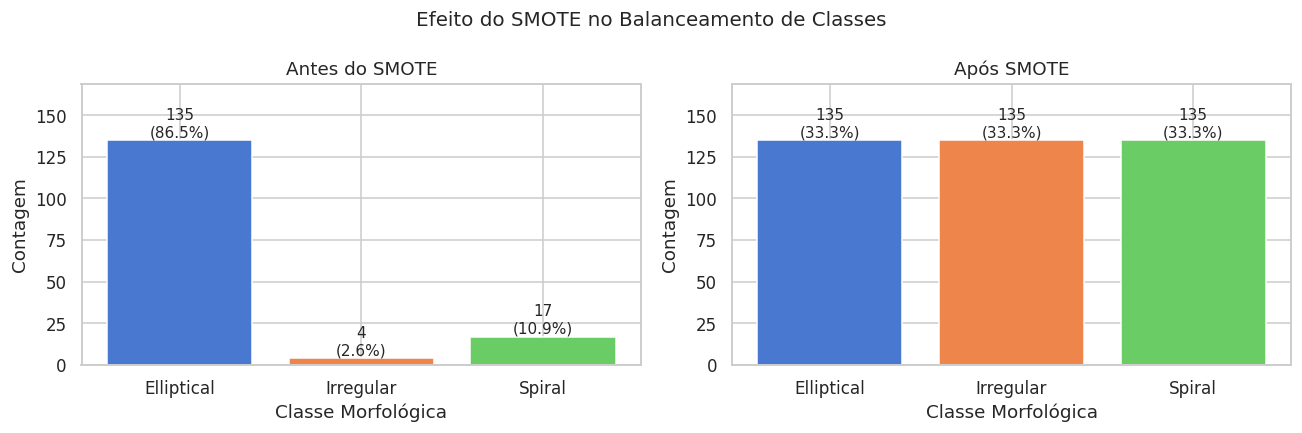
\includegraphics[width=\textwidth]{fig12_smote_balanceamento.png}
  \caption{Distribuição de classes antes e após a aplicação do SMOTE no
           conjunto de treino. O SMOTE equaliza as contagens entre as três
           classes sem duplicar exemplos existentes.}
  \label{fig:smote}
\end{figure}

\textbf{Nota técnica}: com apenas 4~amostras na classe Irregular, o parâmetro
\texttt{k\_neighbors} do SMOTE é ajustado automaticamente para
$k = \max(1,\, N_\text{min} - 1) = 3$ a fim de evitar erro de execução.

\subsection{Artefatos Gerados}

O pré-processamento tabular produz quatro arquivos em \texttt{data/processed/}:

\begin{table}[H]
  \centering
  \caption{Artefatos gerados pelo pré-processamento tabular.}
  \begin{tabular}{llp{7cm}}
    \toprule
    \textbf{Arquivo} & \textbf{Shape / Tipo} & \textbf{Conteúdo} \\
    \midrule
    \texttt{X\_tabular.npy} & $(156, 15)$ \texttt{float32} & Matriz de \textit{features} escalonada \\
    \texttt{y\_labels.npy}  & $(156,)$ \texttt{str} & Rótulos morfológicos \\
    \texttt{objids.npy}     & $(156,)$ \texttt{int64} & \texttt{objid} alinhado com \texttt{X\_tabular} \\
    \texttt{scaler.pkl}     & --- & \texttt{StandardScaler} serializado \\
    \bottomrule
  \end{tabular}
\end{table}

% ─────────────────────────────────────────────────────────────────────────────
\section{Pré-processamento de Imagens (Seção 5.3)}
% ─────────────────────────────────────────────────────────────────────────────

\subsection{Formato das Imagens Brutas}

As imagens FITS foram baixadas do SDSS DR17 via a função
\texttt{download\_galaxy\_image\_cutout()} em \texttt{src/data\_loader.py},
que utiliza a classe \texttt{Cutout2D} do \texttt{astropy} para extrair
recortes centrados na posição de cada galáxia. Cada imagem é armazenada como
um array NumPy de forma $(64, 64, 3)$ e tipo \texttt{float32} nos arquivos
\texttt{data/images/<objid>.npy}, onde os três canais correspondem às bandas
fotométricas $g$, $r$ e $i$ do SDSS (escala de 0,396~arcsec/pixel).

Os valores brutos correspondem a unidades de contagem de fótons do detector
(ADU --- \textit{Analog-to-Digital Units}) após subtração de céu. Sua
distribuição é fortemente assimétrica: o núcleo da galáxia concentra a
maior parte do fluxo, enquanto regiões externas têm valores próximos de zero
ou levemente negativos (ruído).

\subsection{Pipeline de Normalização}

O pipeline é implementado na função
\texttt{preprocess\_galaxy\_image(image\_data, target\_size, stretch\_factor)}
em \texttt{src/preprocessing.py} e aplica, \textbf{por canal independentemente},
três transformações sequenciais:

\subsubsection{Etapa 1: Arcsinh Stretch}

\begin{equation}
  \hat{x} = \text{arcsinh}\!\left(\frac{x}{\alpha}\right)
\end{equation}

onde $x$ é o valor de fluxo bruto e $\alpha = $ \texttt{stretch\_factor}
(padrão: 1000). A função arcsinh possui comportamento linear para $|x| \ll
\alpha$ e logarítmico para $|x| \gg \alpha$, o que:
\begin{itemize}[leftmargin=2em]
  \item \textbf{Realça feições tênues}: braços espirais, disco externo,
        satélites --- regiões de baixo fluxo que o escalonamento linear
        enviaria para próximo de zero.
  \item \textbf{Comprime o núcleo brilhante}: evita a saturação das camadas
        da CNN pelos pixels centrais de alta intensidade.
  \item \textbf{Trata valores negativos}: ao contrário do logaritmo, o arcsinh
        é definido para $x < 0$, manuseando naturalmente o ruído de subtração
        de céu.
\end{itemize}

Esta normalização é padrão em pipelines de processamento de imagens
astronômicas, sendo adotada por projetos como o HSC-SSP e o LSST
\cite{lupton2004}.

\subsubsection{Etapa 2: Escalonamento Min-Max para [0, 1]}

\begin{equation}
  x' = \frac{\hat{x} - \min(\hat{x})}{\max(\hat{x}) - \min(\hat{x})}
\end{equation}

O escalonamento é realizado por canal individualmente, garantindo que cada
banda ocupe todo o intervalo $[0, 1]$ independentemente da sua sensibilidade
absoluta. Canais uniformes (ex.: borda de imagem parcial) são definidos como
zero.

\subsubsection{Etapa 3: Redimensionamento com OpenCV}

O redimensionamento para o tamanho-alvo $(64 \times 64)$ pixels é feito com
\texttt{cv2.INTER\_AREA}, que realiza anti-aliasing médio por blocos e é
preferível ao \texttt{INTER\_LINEAR} para \textit{downscaling}, pois preserva
a energia total da imagem.

\begin{lstlisting}[caption={Implementação do pipeline de pré-processamento de imagens.}, label=lst:preproc_img]
def preprocess_galaxy_image(image_data, target_size=(64,64), stretch_factor=1000):
    if image_data is None:
        return None
    normalized_channels = []
    for i in range(image_data.shape[-1]):
        channel  = image_data[:, :, i]
        stretched = np.arcsinh(channel / stretch_factor)
        ch_min, ch_max = stretched.min(), stretched.max()
        if ch_max - ch_min > 0:
            stretched = (stretched - ch_min) / (ch_max - ch_min)
        else:
            stretched = np.zeros_like(stretched)
        normalized_channels.append(stretched)
    normalized_image = np.stack(normalized_channels, axis=-1)
    # cv2.resize usa (width, height), inverso do numpy
    resized = cv2.resize(normalized_image,
                         (target_size[1], target_size[0]),
                         interpolation=cv2.INTER_AREA)
    return resized.astype(np.float32)
\end{lstlisting}

\subsection{Análise Visual do Pipeline}

A Figura~\ref{fig:raw_vs_proc} compara, canal a canal, a imagem bruta com a
imagem pré-processada para uma galáxia representativa. Observa-se que:
\begin{itemize}[leftmargin=2em]
  \item Na imagem bruta, o contraste dinâmico é dominado pelo núcleo.
  \item Após o \textit{arcsinh stretch}, a estrutura do envelope externo
        da galáxia torna-se visível mesmo em bandas de menor sensibilidade.
  \item A escala de cores na imagem processada cobre uniformemente $[0,1]$
        nos três canais.
\end{itemize}

\begin{figure}[H]
  \centering
  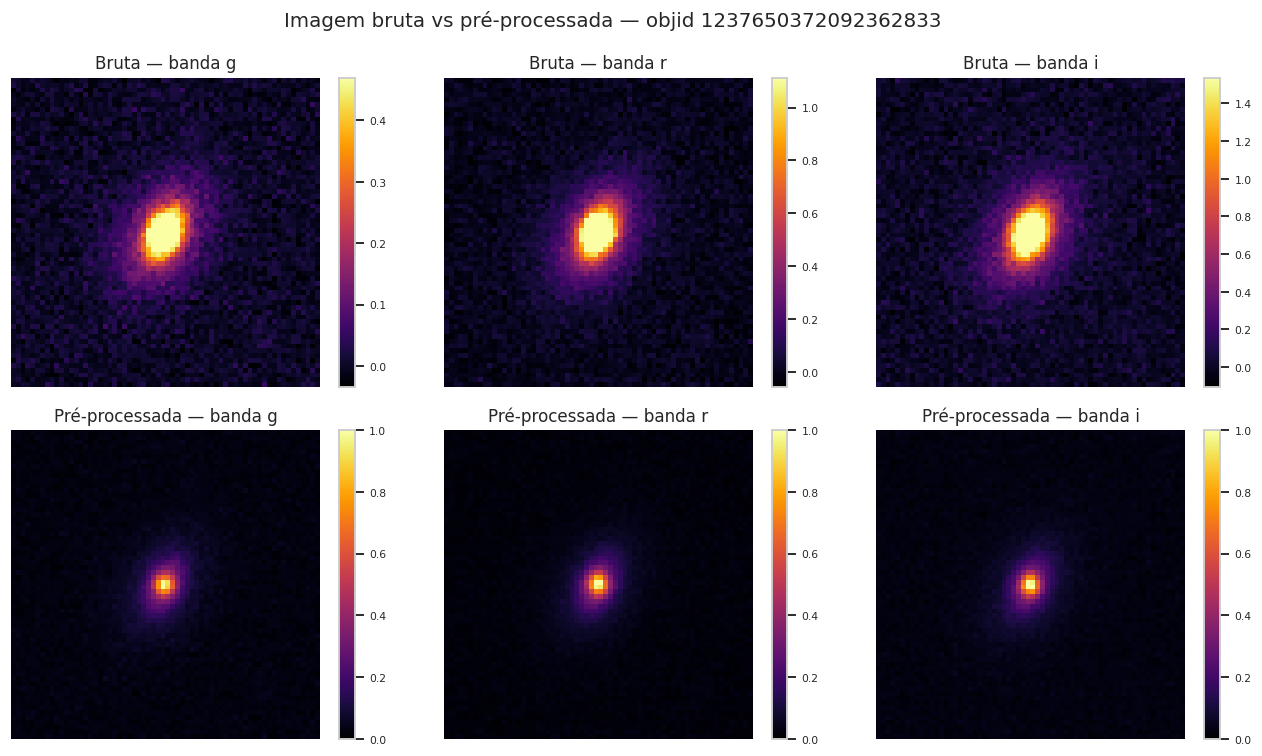
\includegraphics[width=\textwidth]{fig13_raw_vs_processed.png}
  \caption{Comparação entre imagem bruta (linha superior) e pré-processada
           (linha inferior) para os três canais $g$, $r$ e $i$.}
  \label{fig:raw_vs_proc}
\end{figure}

\subsection{Escolha do Parâmetro stretch\_factor}

O parâmetro $\alpha$ (\texttt{stretch\_factor}) controla o ponto de transição
entre o regime linear e o logarítmico do arcsinh. A Figura~\ref{fig:stretch}
ilustra o efeito de diferentes valores de $\alpha$ sobre a banda $r$.

\begin{figure}[H]
  \centering
  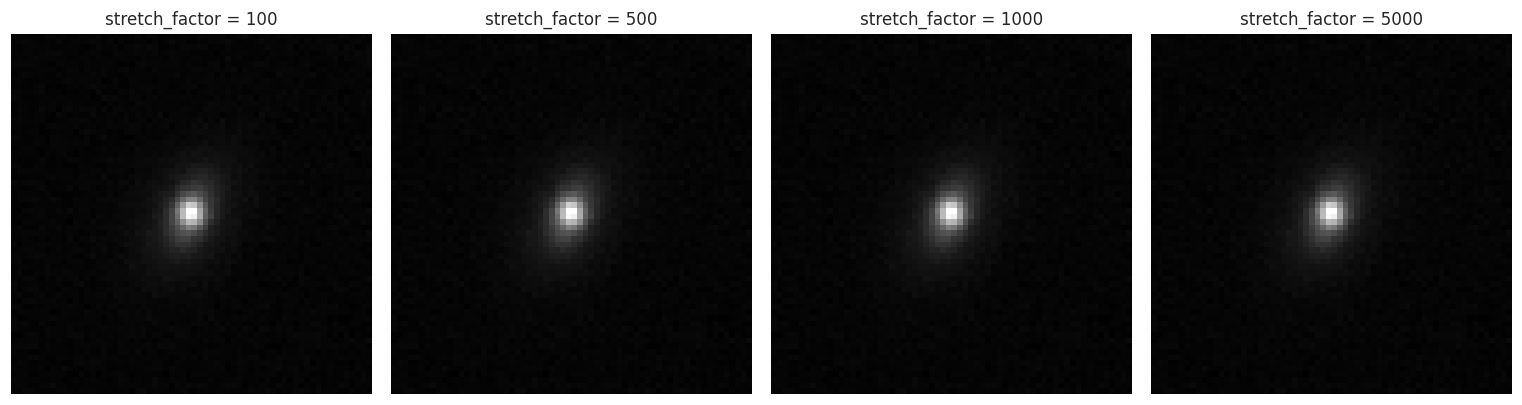
\includegraphics[width=\textwidth]{fig14_stretch_factor.png}
  \caption{Efeito do \texttt{stretch\_factor} na aparência visual da banda $r$.
           Valores menores produzem maior contraste nas regiões tênues; valores
           maiores aproximam-se da escala linear.}
  \label{fig:stretch}
\end{figure}

Valores muito baixos ($\alpha \sim 100$) exageram o ruído de fundo; valores
muito altos ($\alpha \sim 5000$) aproximam-se da escala linear, perdendo a
vantagem do \textit{stretch}. O valor padrão $\alpha = 1000$ representa um
compromisso adequado para imagens SDSS com exposições de $\sim54$~s por banda.

\subsection{Visualização por Classe Morfológica}

A Figura~\ref{fig:grid} apresenta amostras representativas de cada classe em
composição RGB falsa-cor ($r \to R$, $g \to G$, $i \to B$). As diferenças
morfológicas são perceptíveis:

\begin{itemize}[leftmargin=2em]
  \item \textbf{Elípticas}: perfil de brilho suave, sem estrutura interna,
        forma elipsoidal regular.
  \item \textbf{Espirais}: disco estendido, braços ou assimetrias visíveis.
  \item \textbf{Irregulares}: morfologia fragmentada ou assimétrica.
\end{itemize}

\begin{figure}[H]
  \centering
  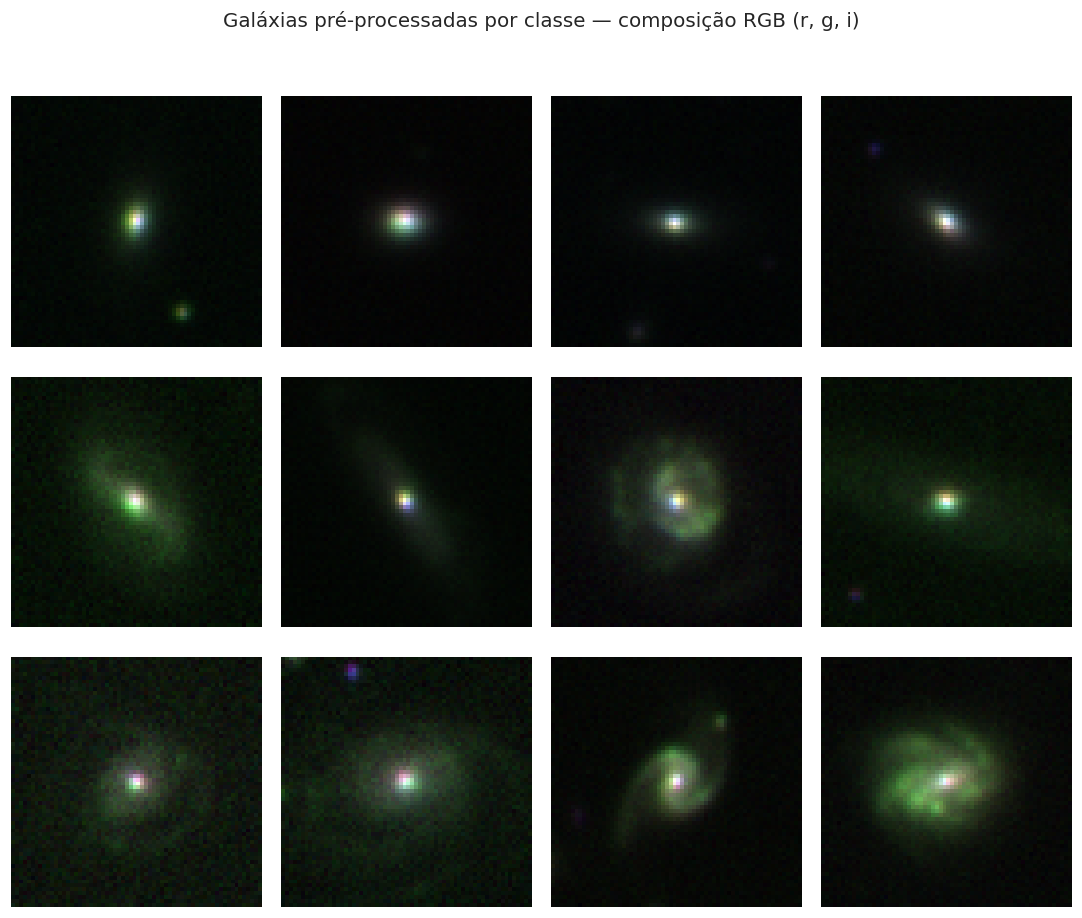
\includegraphics[width=\textwidth]{fig15_galaxy_grid_preprocessed.png}
  \caption{Grid de galáxias pré-processadas por classe morfológica,
           em composição RGB falsa-cor ($r$, $g$, $i$). Cada linha
           corresponde a uma classe; cada coluna, a uma galáxia distinta.}
  \label{fig:grid}
\end{figure}

\subsection{Artefatos Gerados}

O pré-processamento de imagens produz dois arquivos em \texttt{data/processed/}:

\begin{table}[H]
  \centering
  \caption{Artefatos gerados pelo pré-processamento de imagens.}
  \begin{tabular}{llp{7.5cm}}
    \toprule
    \textbf{Arquivo} & \textbf{Shape / Tipo} & \textbf{Conteúdo} \\
    \midrule
    \texttt{X\_images.npy}   & $(N, 64, 64, 3)$ \texttt{float32} & Imagens normalizadas para $[0,1]$ \\
    \texttt{img\_objids.npy} & $(N,)$ \texttt{int64}              & \texttt{objid} alinhado com \texttt{X\_images} \\
    \bottomrule
  \end{tabular}
\end{table}

onde $N$ é o número de galáxias com imagem disponível (imagens ausentes são
ignoradas durante o processamento em lote, com relatório das omissões).

% ─────────────────────────────────────────────────────────────────────────────
\section{Estrutura do Código}
% ─────────────────────────────────────────────────────────────────────────────

O código foi organizado em módulos reutilizáveis em \texttt{src/} e
\textit{scripts} de execução na raiz do projeto (Tabela~\ref{tab:estrutura}).

\begin{table}[H]
  \centering
  \caption{Arquivos implementados até o momento.}
  \label{tab:estrutura}
  \begin{tabular}{lp{9cm}}
    \toprule
    \textbf{Arquivo} & \textbf{Responsabilidade} \\
    \midrule
    \texttt{download\_sdss.py}       & Download de fotometria SDSS DR17 via SQL \\
    \texttt{load\_gz2\_and\_merge.py} & Carregamento do GZ2, \textit{cross-match} e atribuição de classes \\
    \texttt{download\_images.py}     & Download em lote de imagens FITS \\
    \texttt{src/data\_loader.py}     & Funções de acesso aos dois \textit{datasets} e download de imagens \\
    \texttt{src/preprocessing.py}   & Feature engineering, escalonamento e pré-processamento de imagens \\
    \texttt{notebooks/01\_eda.ipynb} & Análise exploratória completa (6 figuras) \\
    \texttt{notebooks/02\_preprocessing.ipynb} & Pré-processamento tabular e de imagens (9 figuras) \\
    \bottomrule
  \end{tabular}
\end{table}

\subsection{Bibliotecas Python Utilizadas}

O projeto foi desenvolvido inteiramente em Python e utiliza um conjunto de
bibliotecas científicas de código aberto, listadas na
Tabela~\ref{tab:bibliotecas}. A seguir, descreve-se o papel de cada uma no
\textit{pipeline}.

\begin{longtable}{lp{10.5cm}}
  \caption{Bibliotecas Python utilizadas no projeto e suas funções.}
  \label{tab:bibliotecas} \\
  \toprule
  \textbf{Biblioteca} & \textbf{Descrição e uso no projeto} \\
  \midrule
  \endfirsthead
  \toprule
  \textbf{Biblioteca} & \textbf{Descrição e uso no projeto} \\
  \midrule
  \endhead
  \bottomrule
  \endfoot

  \texttt{NumPy}
  & Biblioteca fundamental para computação numérica em Python. Fornece o
    objeto \texttt{ndarray} para manipulação eficiente de arrays
    multidimensionais. No projeto, é usada para armazenar e operar sobre
    matrizes de \textit{features} tabulares, imagens de galáxias
    (arrays \texttt{float32} de forma $64 \times 64 \times 3$) e para
    realizar operações matemáticas vetorizadas como o \textit{arcsinh
    stretch} e o escalonamento min-max. \\[6pt]

  \texttt{Pandas}
  & Biblioteca de análise e manipulação de dados tabulares, baseada no
    conceito de \texttt{DataFrame}. Utilizada para carregar, filtrar,
    mesclar e inspecionar os catálogos SDSS e Galaxy Zoo~2 em formato CSV,
    bem como para calcular estatísticas descritivas, tratar valores
    ausentes (\texttt{dropna}) e gerar as colunas derivadas (índices de
    cor, concentração). \\[6pt]

  \texttt{Astropy}
  & Pacote central da comunidade astronômica Python. No projeto, são
    utilizados os seguintes submódulos:
    \texttt{astropy.coordinates.SkyCoord} para representar coordenadas
    celestes e executar o cruzamento espacial (\textit{cross-match}) entre
    SDSS e GZ2;
    \texttt{astropy.units} para conversão de unidades angulares (graus,
    arcsec);
    \texttt{astropy.io.fits} para leitura de arquivos FITS;
    \texttt{astropy.nddata.Cutout2D} para extrair recortes centrados na
    posição de cada galáxia; e
    \texttt{astropy.wcs.WCS} para converter coordenadas celestes em
    coordenadas de pixel. \\[6pt]

  \texttt{Astroquery}
  & Pacote afiliado ao Astropy que fornece interfaces Python para consultar
    bancos de dados astronômicos remotos. O submódulo
    \texttt{astroquery.sdss.SDSS} é utilizado para enviar consultas SQL
    ao \textit{SkyServer} do SDSS DR17 e para baixar imagens FITS das
    galáxias via a função \texttt{SDSS.get\_images()}. \\[6pt]

  \texttt{Matplotlib}
  & Biblioteca padrão de visualização científica em Python. Utilizada
    para gerar todas as figuras do projeto: histogramas de distribuição
    de classes e \textit{redshift}, diagramas de cor-magnitude,
    \textit{heatmaps} de correlação, grids de imagens de galáxias e
    comparações visuais entre imagens brutas e pré-processadas. \\[6pt]

  \texttt{Seaborn}
  & Biblioteca de visualização estatística construída sobre o Matplotlib.
    Facilita a criação de gráficos como \textit{boxplots} por categoria,
    matrizes de correlação com anotações (\texttt{heatmap}), histogramas
    com separação por classe (\texttt{histplot} com \texttt{hue}) e
    diagramas de dispersão com paletas de cores categóricas. \\[6pt]

  \texttt{Scikit-learn}
  & Biblioteca de aprendizado de máquina de propósito geral. No projeto,
    são utilizados:
    \texttt{StandardScaler} para normalização das \textit{features}
    tabulares (média zero, variância unitária);
    \texttt{LabelEncoder} para codificação dos rótulos morfológicos em
    inteiros; e
    \texttt{train\_test\_split} para partição dos dados em conjuntos de
    treino, validação e teste com estratificação por classe. \\[6pt]

  \texttt{Imbalanced-learn}
  & Extensão do Scikit-learn voltada para problemas com desbalanceamento
    de classes. A técnica \textbf{SMOTE} (\textit{Synthetic Minority
    Over-sampling Technique}) é utilizada para gerar amostras sintéticas
    das classes minoritárias (Spiral e Irregular) no espaço de
    \textit{features}, equilibrando as contagens de treino sem duplicar
    exemplos reais. \\[6pt]

  \texttt{OpenCV}
  & Biblioteca de visão computacional de alto desempenho (módulo
    \texttt{cv2} em Python). Utilizada exclusivamente para o
    redimensionamento das imagens de galáxias com interpolação
    \texttt{INTER\_AREA}, que realiza subamostragem por média de blocos
    e é o método preferível para \textit{downscaling}, pois preserva a
    energia total da imagem sem introduzir artefatos de
    \textit{aliasing}. \\[6pt]

  \texttt{SciPy}
  & Biblioteca de algoritmos científicos e matemáticos. Serve como
    dependência interna do Astropy e do Scikit-learn, fornecendo rotinas
    de álgebra linear, interpolação e otimização. \\[6pt]

  \texttt{TensorFlow / Keras}
  & \textit{Framework} de \textit{Deep Learning} que será utilizado nas
    próximas etapas do projeto para definir, treinar e avaliar as três
    arquiteturas de redes neurais: MLP (\textit{Multi-Layer Perceptron}),
    CNN (\textit{Convolutional Neural Network}) e o modelo Híbrido de
    dupla entrada. A API \texttt{tf.keras} fornece camadas como
    \texttt{Dense}, \texttt{Conv2D}, \texttt{BatchNormalization} e
    \texttt{Dropout}, além de \textit{callbacks} como
    \texttt{EarlyStopping} e \texttt{ModelCheckpoint}. \\[6pt]

  \texttt{Photutils}
  & Pacote afiliado ao Astropy para fotometria de fontes astronômicas.
    Disponível no ambiente para análise de abertura e detecção de fontes,
    podendo ser utilizado em etapas futuras de extração de
    \textit{features} morfométricas diretamente das imagens. \\[6pt]

  \texttt{tqdm}
  & Biblioteca que fornece barras de progresso para iterações longas.
    Utilizada no download em lote de imagens FITS
    (\texttt{download\_images\_batch}) para exibir o progresso e o tempo
    estimado de conclusão em tempo real. \\

\end{longtable}

% ─────────────────────────────────────────────────────────────────────────────
\section{Próximas Etapas}
% ─────────────────────────────────────────────────────────────────────────────

Com a base de dados preparada, as próximas fases do projeto são:

\begin{enumerate}[leftmargin=2em]
  \item \textbf{Modelo MLP} (\texttt{03\_mlp\_model.ipynb}): carregar
        \texttt{X\_tabular.npy} e \texttt{y\_labels.npy}, aplicar SMOTE
        somente no treino, definir e treinar a arquitetura Sequential com
        camadas Dense-BatchNorm-Dropout, e avaliar com métricas de
        \textit{Completeness} e \textit{Reliability}.

  \item \textbf{Modelo CNN} (\texttt{04\_cnn\_model.ipynb}): carregar
        \texttt{X\_images.npy}, aplicar \textit{data augmentation} com
        \texttt{ImageDataGenerator} (\texttt{rotation\_range=360},
        \textit{flips}, \textit{zoom}), e treinar a arquitetura de quatro
        blocos convolucionais.

  \item \textbf{Modelo Híbrido} (\texttt{05\_hybrid\_model.ipynb}): fusão
        do ramo CNN e do ramo MLP via concatenação de vetores de
        \textit{feature}, treinamento conjunto e análise de
        \textit{Grad-CAM} para interpretabilidade.

  \item \textbf{Avaliação Científica}: geração de matrizes de confusão,
        comparação dos três modelos e discussão das implicações astrofísicas
        dos erros de classificação.
\end{enumerate}

% ─────────────────────────────────────────────────────────────────────────────
\section{Conclusão Parcial}
% ─────────────────────────────────────────────────────────────────────────────

As etapas de aquisição de dados, EDA e pré-processamento foram concluídas
com sucesso, produzindo um catálogo limpo de 156~galáxias com rótulos
confiáveis, 15~\textit{features} tabulares normalizadas e imagens
$64 \times 64 \times 3$ em $[0,1]$. Os principais desafios identificados
são o severo desbalanceamento de classes (86,5\% elípticas) e o tamanho
reduzido do conjunto de dados, que exigirão técnicas de regularização e
aumento de dados (\textit{data augmentation}) nas fases de modelagem.

% ─────────────────────────────────────────────────────────────────────────────
\begin{thebibliography}{9}

\bibitem{hart2016}
Hart, R.~E. et al. (2016).
\textit{Galaxy Zoo 2: detailed morphological classifications for 304,122 galaxies from the Sloan Digital Sky Survey}.
Monthly Notices of the Royal Astronomical Society, 445(4), 3466--3486.
\url{https://doi.org/10.1093/mnras/stu1816}

\bibitem{conselice2003}
Conselice, C.~J. (2003).
\textit{The Relationship between Stellar Light Distributions of Galaxies and Their Formation Histories}.
The Astrophysical Journal Supplement Series, 147(1), 1--28.
\url{https://doi.org/10.1086/375001}

\bibitem{chawla2002}
Chawla, N.~V., Bowyer, K.~W., Hall, L.~O., \& Kegelmeyer, W.~P. (2002).
\textit{SMOTE: Synthetic Minority Over-sampling Technique}.
Journal of Artificial Intelligence Research, 16, 321--357.
\url{https://doi.org/10.1613/jair.953}

\bibitem{lupton2004}
Lupton, R., Blanton, M.~R., Fekete, G., et al. (2004).
\textit{Preparing Red-Green-Blue Images from CCD Data}.
Publications of the Astronomical Society of the Pacific, 116(816), 133--137.
\url{https://doi.org/10.1086/382245}

\bibitem{sdss_dr17}
Abdurrouf et al. (2022).
\textit{The Seventeenth Data Release of the Sloan Digital Sky Surveys: Complete Release of MaNGA, MaStar, and APOGEE-2 Data}.
The Astrophysical Journal Supplement Series, 259(2), 35.
\url{https://doi.org/10.3847/1538-4365/ac4414}

\end{thebibliography}

\end{document}
